\tolerance=10000
\documentclass{book}
\usepackage{amsmath,times,graphicx,url,verbatim,mcode}
\usepackage{tikz}
\usetikzlibrary{shapes,arrows}
\tikzstyle{block} = [draw, fill=blue!20, rectangle, 
    minimum height=3em, minimum width=6em]
\tikzstyle{sum} = [draw, fill=blue!20, circle, node distance=1cm]
\tikzstyle{pinstyle} = [pin edge={to-,thin,black}]
%\pgfsysdriver{pgfsys-tex4ht.def} 

\newcommand{\pd}[2]{\frac{\partial #1}{\partial #2}}
\newcommand{\bq}{{\bf q}}
\newcommand{\bx}{{\bf x}}
\newcommand{\bu}{{\bf u}}
\newcommand{\bw}{{\bf w}}
\newcommand{\bz}{{\bf z}}
\newcommand{\bK}{{\bf K}}
\newcommand{\balpha}{{\bf \alpha}}
\newcommand{\bbeta}{{\bf \beta}}
\newcommand{\avg}[1]{E\left[ #1 \right]}
\DeclareMathOperator*{\argmin}{argmin}
\DeclareMathOperator*{\sgn}{sgn}

\usepackage{xspace}
\newcommand{\robotlib}{RobotLib\xspace}
\newcommand{\matlab}{MATLAB\xspace}
\newcommand{\simulink}{Simulink\xspace}
\newtheorem{example}{Example}

\usepackage{xcolor}
% switch to other comment command to remove all comments.
\newcommand{\todo}[1]{\marginpar{\tiny\color{blue}#1\raggedright}}


\title{\Huge \robotlib Documentation}
\author{\Large Robot Locomotion Group}

\begin{document}
\maketitle

\tableofcontents 

% preface/intro.  acknowledgements/contributors
% getting help:  help command.  doc command.  doxygen documentation (searchable)

\chapter{Installation and QuickStart}

\chapter{Modeling and Simulation}

The fundamental object in \robotlib is a dynamical system.  Robots, 
controllers, state estimators, etc. are all instances of dynamical
systems.  Algorithms in \robotlib operate on dynamical systems.  This
chapter introduces what you need to know to instantiate the dynamical
systems that you are interested in, and to simulate and visualize
their outputs.  

\section{Modeling Input-Ouput Dynamical Systems}

Dynamical systems in \robotlib are represented by their dynamics in
state-space form, with $x$ denoting the state vector.  In addition,
every dynamical system can have an input vector, $u$, and an output
vector $y$. 

\begin{center}
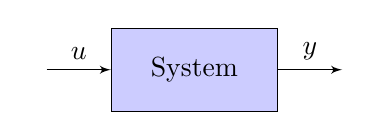
\begin{tikzpicture}[auto, node distance=2cm,>=latex']
   \node (input) {};
   \node [block, right of=input] (system) {System};
   \draw [->] (input) -- node {$u$} (system);
   \node [right of=system] (output) {};
   \draw [->] (system) -- node {$y$} (output);
\end{tikzpicture}
\end{center}

As we will see, dynamical systems in \robotlib can be instantiated in a number of different ways.  A system can be described by a block of C code (see for instance section~\ref{s:simulinksystem}), but many of the algorithms implemented in \robotlib operate symbolically on the governing equations of the dynamical systems.  For this reason, the preferred approach is (for rigid body dynamics) to use the RobotLib URDF interface or alternatively to describe your dynamics in \matlab code by deriving from the RobotLibSystem interface class.


\subsection{Universal Robot Description Format (URDF)}


\subsection{Writing your own dynamics}

Not every system of interest can be described by the URDF interface.  For example, for some simple model systems, it makes more sense to type in the few lines of \matlab code to describe the system.  In other cases, such as modeling a aircraft, there may be terms required in the dynamics (such as aerodynamic forces) that are not programmed into the rigid-body URDF interface.  Similarly, if you need to write your own control system or state estimator, you will need to write your own code.   In this section, we will describe how you can write your own dynamics class by deriving from the RobotLibSystem interface class. 

\subsubsection{Continuous-Time Systems}

Consider a basic continuous-time nonlinear input-output dynamical system described by the following state-space equations:
\begin{gather*}
\dot{x} = f(t,x,u), \\ y = g(t,x,u).
\end{gather*}
In \robotlib, you can instantiate a system of this form where $f()$ and $g()$ are anything that you can write into a \matlab function.  This is accomplished by deriving from the RobotLibSystem class, defining the size of the input, state, and output vectors in the constructor, and overloading the \mcode{dynamics} and \mcode{output} methods, as illustrated by the following example:

\begin{example}[A simple continuous-time system]
Consider the system \begin{gather*}\dot{x} = -x + x^3,\\ y = x.\end{gather*}  This system has zero inputs, one (continuous) state variable, and one output.  It can be implemented in \robotlib using the following code:
\lstinputlisting{../examples/SimpleCTExample.m}
\end{example}


\subsubsection{Discrete-Time Systems}

Implementing a basic discrete-time system in \robotlib is very analogous to implementing a continuous-time system.  The discrete-time system given by:
\begin{gather*}
x[n+1] = f(n,x,u),\\
y[n] = g(n,x,u),
\end{gather*}
can be implemented by deriving from \mcode{RobotLibSystem} and defining the \mcode{update} and \mcode{output} methods, as seen in the following example.  

\begin{example}[A simple discrete-time system]
Consider the system \begin{gather*}x[n+1] = x^3[n],\\ y[n] = x[n].\end{gather*}  This system has zero inputs, one (discrete) state variable, and one output.  It can be implemented in \robotlib using the following code:
\lstinputlisting{../examples/SimpleDTExample.m}
\end{example}


\subsubsection{Mixed Discrete and Continous Dynamics}

It is also possible to implement systems that have both continuous
dynamics and discrete dynamics.  There are two subtleties that must be
addressed.  First, we'll denote the discrete states as $x_d$ and the
continuous states as $x_c$, and the entire state vector $x = [x_d^T,
x_c^T]^T$.  Second, we must define the timing of the discrete dynamics
update relative to the continuous time variable $t$; we'll denote this
period with $\Delta_t$.  Then a mixed system can be written
as:\begin{gather*} \dot{x}_c = f_c(t,x,u),\\ x_d(t+t') = f_d(t,x,u),
  \quad \forall t \in \{0,\Delta_t,2\Delta_t,...\},\forall t' \in
  (0,\Delta_t] \\ y=g(t,x,u). \end{gather*} Note that, unlike the
purley discrete time example, the solution of the discrete time variable is defined
for all $t$.  To implement this, derive from RobotLibSystem and
implement the \mcode{dynamics}, \mcode{update}, \mcode{output} methods
for $f_c()$, $f_d()$, and $g()$, respectively.  To define the timing,
you must also implement the \mcode{getSampleTime} method.  Type
\mcode{help RobotLibSystem/getSampleTime} at the \matlab prompt for
more information.

\begin{example}[A mixed discrete- and continuous-time example]
Consider the system \begin{gather*}x_1(t+t') = x_1^3(t), \quad \forall
  t \in \{0,1,2,..\}, \forall t' \in (0,1], \\\dot{x}_2 =
  -x_2(t) + x_2^3(t), \end{gather*} which is the combination of the
previous two examples into a single system.  It can be implemented in \robotlib using the following code:
\lstinputlisting{../examples/SimpleMixedCTDTExample.m}
\end{example}

\subsubsection{Systems w/ Constraints}

Nonlinear input-output systems with constraints can
also be defined.  There are two distinct types of constraints supported: state constraints that can be modeled as a function $\phi(x) = 0$ and input constraints which can be modeled as $u_{min} \le u \le u_{max}$.  For instance, we would write a continuous-time system with state and input constraints as:
\begin{gather*}
\dot{x} = f(t,x,u),\quad y = g(t,x,u), \\ \text{subject to }  \phi(x) =
0, u_{min} \le u \le u_{max}.
\end{gather*}
These two types of constraints are handled quite differently.  

Input constraints are designed to act in the same way that an actuator limit might work for a mechanical system.  These act as a saturation nonlinearity system attached to the input, where for each element: $$y_i = \begin{cases} u_{max,i} & \text{if } u_i > u_{max,i} \\ u_{min,i} & \text{if } u_i < u_{min,i} \\ u_i & \text{otherwise.}\end{cases}$$  The advantage of using the input limits instead of implementing the saturation in your own code is that the discontinuity associated with hitting or leaving a saturation is communicated to the solver correctly, allowing for more efficient and accurate simulations.  Input constraints are set by calling the \mcode{setInputLimits} method.  

State constraints are additional information that you are providing to the solver and analysis routines.  They should be read as ``this dynamical system will only ever visit states described by $\phi(x)=0$''.  Evaluating the dynamics at a vector $x$ for which $\phi(x) \ne 0$ may lead to an undefined or non-sensible output.   Telling \robotlib about this constraint will allow it to select initial conditions which satisfy the constraint, simulate the system more accurately (with the constraint imposed), and restrict attention during analysis to the manifold defined by the constraints.  However, \emph{the state constraints function should not be used to enforce an additional constraint that is not already imposed on the system by the governing equations.}.  The state constraint should be simply announcing a property that the system already has, if simulated accurately.   Examples might include a passive system with a known total energy, or a four-bar linkage in a rigid body whos dynamics are written as a kinematic tree + constraint forces.   State constraints are implemented by overloading the \mcode{stateConstraints} method \emph{and} by calling \mcode{setNumStateConstraints} to tell the solver what to expect in that method.  
 
\todo{implement example of passive pendulum with and without state constraints, showing the additional accuracy.}

\subsubsection{Event-Driven Systems}

Event-based hybrid systems


\subsubsection{Stochastic Systems}


\subsubsection{Important Special Cases} \label{s:system_subclasses}

There are many special cases of smooth systems with structure in the
dynamics which can be exploited by our algorithms.  Special cases of
smooth dynamical systems implemented in RobotLib include
\begin{itemize}
\item Smooth systems.  Any mixture of continuous and discrete time dynamics, where the functions governing the dynamics ($f(), g(),$ ...) are smooth functions.  Smooth functions are functions that are continuous with derivatives that exist everywhere  and are smooth\cite{wiki:Smooth_Function}.   
\item Piecewise-smooth systems. 
\item Second-order systems, given by $\ddot{q} = f(t,q,\dot{q},u),$ $y
  = g(t,q,\dot{q},u)$, and $\phi_1(q)=0$ and $\phi_2(q,\dot{q})=0$.  
\item Rigid-body systems, governed by the manipulator
  equations, \begin{gather*}H(q)\ddot{q} + C(q,\dot{q})\dot{q} + G(q) = Bu + \pd{\phi_1}{q}^T
  \lambda_1 + \pd{\phi_2}{\dot{q}}^T \lambda_2\\ \phi_1(q) = 0, \quad
  \phi_2(q,\dot{q})=0\end{gather*} where $\lambda_1$ and $\lambda_2$
are forces defined implicitly by the constraints.   
\item URDF.  Derive from, but add initial conditions, etc.
\item (Rational) polynomial systems, given by $e(x)\dot{x} =
  f(t,x,u)$, $y = g(t,x,u)$, subject to $\phi(x)=0$, where $e(), f(),
  g(),$ and $\phi()$ are all polynomial.  \todo{also discrete time}
%% better not to mention these here:
%\item Polynomial trajectory systems \todo{Is there a better name for
%   these systems?}, given by $\dot{x} = f(t,x,u)$,
%  $y=g(t,x,u)$, where $f()$ and $g()$ are polynomial in $x$ and $u$,
%  but not necessarily in $t$.  
\item Linear time-invariant systems, given by $\dot{x} = Ax + Bu,$
  $y=Cx + Du$, and $\phi(x)=\{\}$.  \todo{also discrete time}
\end{itemize}
These special cases are implemented by classes derived from SmoothRobotLibSystem.
You should always attempt to derive from the deepest class in the hierarchy that
describes your system.  


Some of the algorithms available for simulation and
analysis of dynamical systems need to make assumptions about the
smoothness of the equations governing the dynamics of the systems they
are operating on.  For this reason, the methods for implementing
dynamical systems are designed to force you to be explicit about when
these smoothness assumptions are valid.  


In some cases it is possible to convert between these derived
classes.  For example, converting a rigid-body system to a rational
polynomial system (e.g., by changing coordinates through a
stereographic projection).  Methods which implement these conversions are
provided whenever possible.  

Todo: xcubed example again, but this time deriving from polynomialsystem.  


\subsubsection{Providing User Gradients}


\subsection{Existing \simulink Models/Blocks}\label{s:simulinksystem}

Although most users of RobotLib never open a \simulink GUI, \robotlib
is built on top of the \matlab \simulink engine.  As such, \robotlib
systems can be used in any \simulink model, and any existing \simulink
block or \simulink model (an entire \simulink diagram) which has a
single (vector) input and single (vector) output can be used with the
\robotlib infrastructure.  

\subsection{Combinations of Systems}

\begin{figure}[h]
\begin{center}
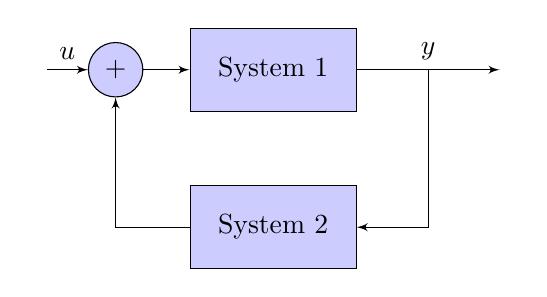
\begin{tikzpicture}[auto, node distance=2cm,>=latex']
    % We start by placing the blocks
    \node (input) {};
    \node [sum, right of=input] (sum) {$+$};
    \node [block, right of=sum] (sys1) {System 1};
    \node [block, below of=sys1] (sys2) {System 2};
    \node [right of=sys1, node distance=3cm] (output) {};
    \draw [->] (input) -- node{$u$} (sum);
    \draw [->] (sum) -- (sys1);
    \draw [->] (sys1) -- node(y){$y$} (output);
    \draw [->] (y) |- (sys2);
    \draw [->] (sys2) -| (sum);
\end{tikzpicture}
\end{center}
\caption{Feedback combination}
\end{figure}

\begin{figure}[h]
\begin{center}
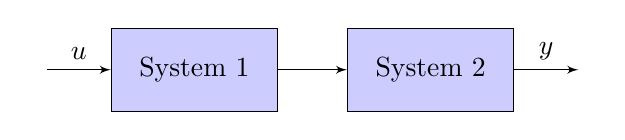
\begin{tikzpicture}[auto, node distance=2cm,>=latex']
    % We start by placing the blocks
    \node (input) {};
   \node [block, right of=input] (sys1) {System 1};
   \node [block] (sys2) at +(5,0) {System 2};
   \node [right of=sys2] (output) {};
   \draw [->] (input) -- node{$u$} (sys1);
   \draw [->] (sys1) -- (sys2);
   \draw [->] (sys2) -- node(y){$y$} (output);
\end{tikzpicture}
\end{center}
\caption{Cascade combination}
\end{figure}

Whenever possible, structure in the equations is preserved on
combination.  A polynomial system that is feedback combined with
another polynomial system produces a new polynomial system.   However,
if a polynomial system is feedback combined with a \simulink Block,
then the new system is a DynamicalSystem, but not a PolynomialSystem.  

\section{Simulation}

The simulate command.

Simulation options.  

The realtime block.

Zero crossings.

setting default initial conditions.

\section{Visualization}

Playback

Cascading.   Use the realtime block.

\subsection{Outputing to a movie format}



\chapter{Analysis}

\section{Fixed Points}

\subsection{Local Stability}

\subsection{Global Stability}

\subsection{Regions of Attraction}

\section{Limit Cycles}

\subsection{Local Stability}

\subsection{Regions of Attraction}

\section{Trajectories}

\subsection{Finite-time invariant regions}


\chapter{Planning}

\chapter{Feedback Design}

\chapter{System Identification}

\chapter{State Estimation}

\chapter{External Interfaces}

Controlling real robots. 

\bibliographystyle{plain}
\bibliography{local} %,elib

\end{document}
